%!TEX root = main.tex
\section{Dataset}
På de følgende sider vil vi gennnemgå vores dataset. Vi vil vise de basale statistikker over dataet og gennemgå afvigelser. Vi vil også gennemgå hvordan vi forholder os til disse afvigelser og hvordan vi lavede datacleaning. \\

Vores data stammer fra Sony's Lifelog\cite{sonyLifeLog} som navnet antyder, er en mobil Lifelog app som logger ens aktiviteter i løbet af dagen. Heri logger den bla. aktivitet i apps og geolokation. Vores dataset stammer fra denne app, indsamlet fra 1586 Sony medarbejdere over 3 måneder\footnote{September 2015 - November 2015} fordelt på 80 lande. 

Vi kan dele datasettet op i 2 dele for oveblikkets skyld: En \textbf{geolokation del} og en \textbf{app og homophily del}. \\


\textbf{Geolokation del}\\
I denne del ligger det mest interessante i forhold til vores problemstilling. Dette er geolokationen for brugeren på et pågældende tidspunkt. Lokationen bliver logget når lokationen ændre sig (værdierne for latitude eller longitude ændre sig). Når lokationen bliver logget, bliver et time stamp også logget (\texttt{start\_time}) - og når lokationen ændre sig, bliver et andet time stamp logget (\texttt{end\_time}). Dvs. at \texttt{start\_time} og \texttt{end\_time} er ens, så længe brugeren er i bevægelse.

Accuracy af GPS og altitude bliver også logget, samt meta-data for pågældende lokation - city name, country, region and area. Table \ref{tab:stat_geo} viser disse attributter samt nogle nøgle værdier. 

\begin{table}[htbp]
        \centering
        \small
        \setlength\tabcolsep{2pt}
        \begin{tabular}{|c|c|c|c|c|c|c|c|c|c|c|}
            \hline
                         & Latitude/  &   start             & end               & Accuracy           & Altitude    & Name   & Country & Region             & Area          \\[-3pt]% compensate for extrarowheight
                         & longitude  &  time               & time              &  (mm)              & (mm)        & (city) &         & (Europe, Asia...)  & (Area/state)  \\
            \hline
                 Unique  &            &                     &                   &                    &             & 19.344 & 80      &                    &               \\
                 entries &            &                     &                   &                    &             &        &         &                    &               \\
            \hline
                 Min     &            &   2015-08-09        &                   &  -2.147.483.500    & -5.086.000  &        &         &                    &               \\
                         &            &   22:25:33.766+02   &                   &                    &             &        &         &                    &               \\
            \hline
                 Max     &            &                     &   2015-12-01      &  500.000           & 17.211.698  &        &         &                    &               \\
                         &            &                     &  01:00:22.711+01  &                    &             &        &         &                    &               \\
            \hline
                 Mean    &            &                     &                   & 35.249             & 105.030     &        &         &                    &               \\
                         &            &                     &                   &                    &             &        &         &                    &               \\
            \hline
                 Std.    &            &                     &                   & 3.672.390          & 403.966     &        &         &                    &               \\
                 dev.    &            &                     &                   &                    &             &        &         &                    &               \\
            \hline
        \end{tabular}
        \caption{Overview and statistic summary of geolocation dataset} %add this between 'caption' and '{...' for new text in listing of tables: [New caption text only for listing of tables]
        \label{tab:stat_geo}
\end{table}

Vi kan se i tabellen at der er nogle ugyldige værdier såsom negative accuracy. Ud af de 2.665.893 records er der kun 20 hvor accuracy er negativ hvilket svarer til knapt en 1000 del procent. Altitude har også nogle negative værdier. Her er negative værdier ikke ugyldige, men dog sjældne og unormale. Hvis vi kigger på antal records de har en negativ altitude på mindre end -50.000 (-50m), er der 9. Ved mindre end -10.000 (-10m) er der 14.

I begge attributter opstår de ugyldige/sjældne værdier så sjældent i vores datasæt, at det ikke gør nogen forskel at de bliver fjernet. Specielt ved accuracy som går ud over latitude og longitude, er det vigtigt at fjerne disse, da latitude og longitude er den mest vigtige attribut for projektet. 

I Tabel \ref{tab:stat_geo} kan vi se der er 80 unikke lande. Til at starte med lå dette tal på 74. Det viste sig, at der var en masse records hvor landet ikke var blevet logget. Her var landet blot repræsenteret med en tom streng. Dette var tilfældet i så stor en del af dataet, at landet med en tom streng, var det andet mest representerede land i dataet med lidt over 500.000 records. 
Dette var et problem som vi løste, ved at udfører omvendt geolokation. For næsten alle de 500.000 records, var latitude og longitude til stede, så vi kunne ved hjælp af et API [ref] slå landet op på bagrund af latitude og longitude, og herefter indsætte det i dataet. 
Dette gjorde at vi gik fra over 500.000 records hvor landet ikke var til stede, til blot 130 records. I samme omgang gik vi fra 74 lande til 80 (inkl. land med tom streng)



Vi kunne herefter kigge på hvordan records var distribueret over hvert land. På figur \ref{fig:country_dist} kan vi se at landet med en tom streng, røg godt ned på listen, mens Sverige og Japan topper listen. 
\begin{figure}[H]
    \centering
    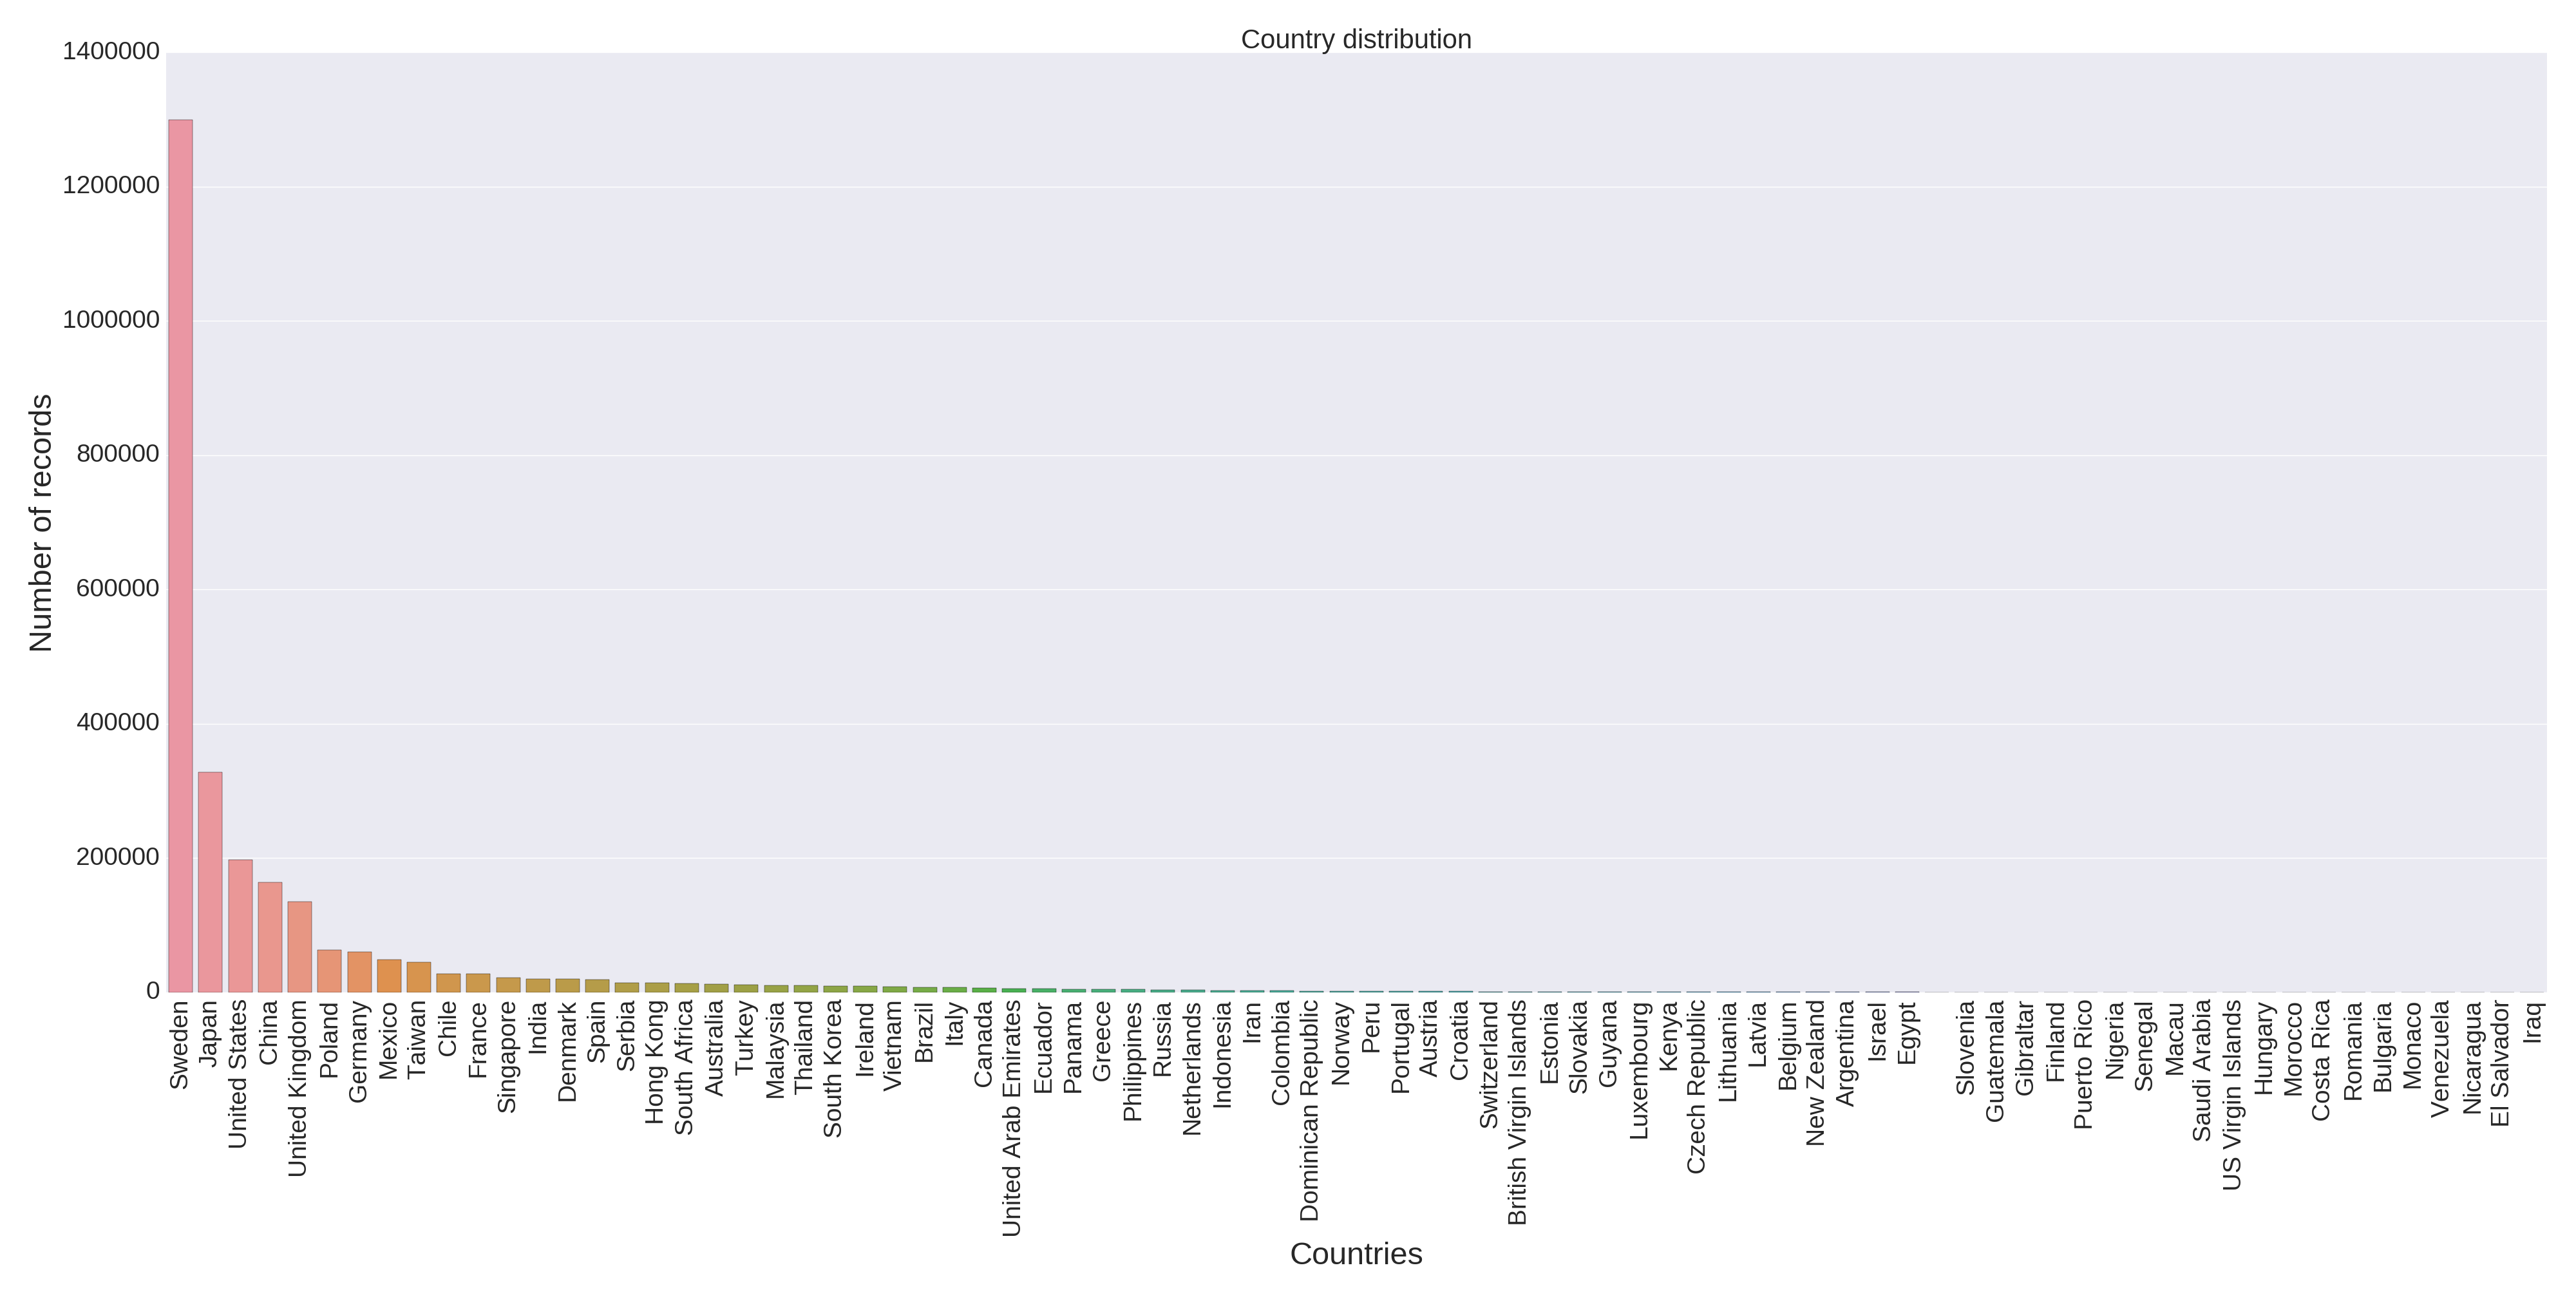
\includegraphics[scale=0.18]{country_distribution}
    \caption{Distribution for number of records between countries}
    \label{fig:country_dist}
\end{figure}

På baggrund af figur \ref{fig:country_dist}, har vi valgt at gå videre med endten Sverige eller Japan. Derfor vil vi nu sammeligne data for de to lande. 
På Figur \ref{fig:country_cd} ser vi at der er en stor del af brugerne både i Japan og Sverige, som har meget få lokations opdateringer henover hele perioden. Over en tredje del af brugerne i begge lande, har maximalt 109 og 161 opdateringer over 3 måneder for henholdsvis Japan og Sverige. Da opdateringerne kommer hver gang brugeren skifter lokation (latitude/longitude skifter- hvor mange meter er det egentligt?), betyder dette at mange af brugerene er meget stillestående eller også har de slukket mobilen. Begge disse scenarier tegner ikke godt for vores mål, da det giver sig selv at der skal være nogle data for at finde co-occurences. 

For at bedre kunne sammenligne Japan og Sverige udfra Figure \ref{fig:country_cd}, har vi plottet den Cumulative Distribution Function (CDF) for de to lande (Figure \ref{fig:country_cdf}). Plottet viser at Japan har flere brugere med få lokations opdateringer end Sverige, mens Sverige har flere opdateringer generelt. Dette kunne tyde på at data fra  Sverige vil være mere brugbart end Japan. Dog er binsize forskellig for de to plot og hvis vi sammenligner nøgleværdierne for de to lande (Table \ref{tab:stat_loc_updates}) kan vi se, at Sverige har større Q1 end Japan.




\begin{figure}[H]
    \centering
    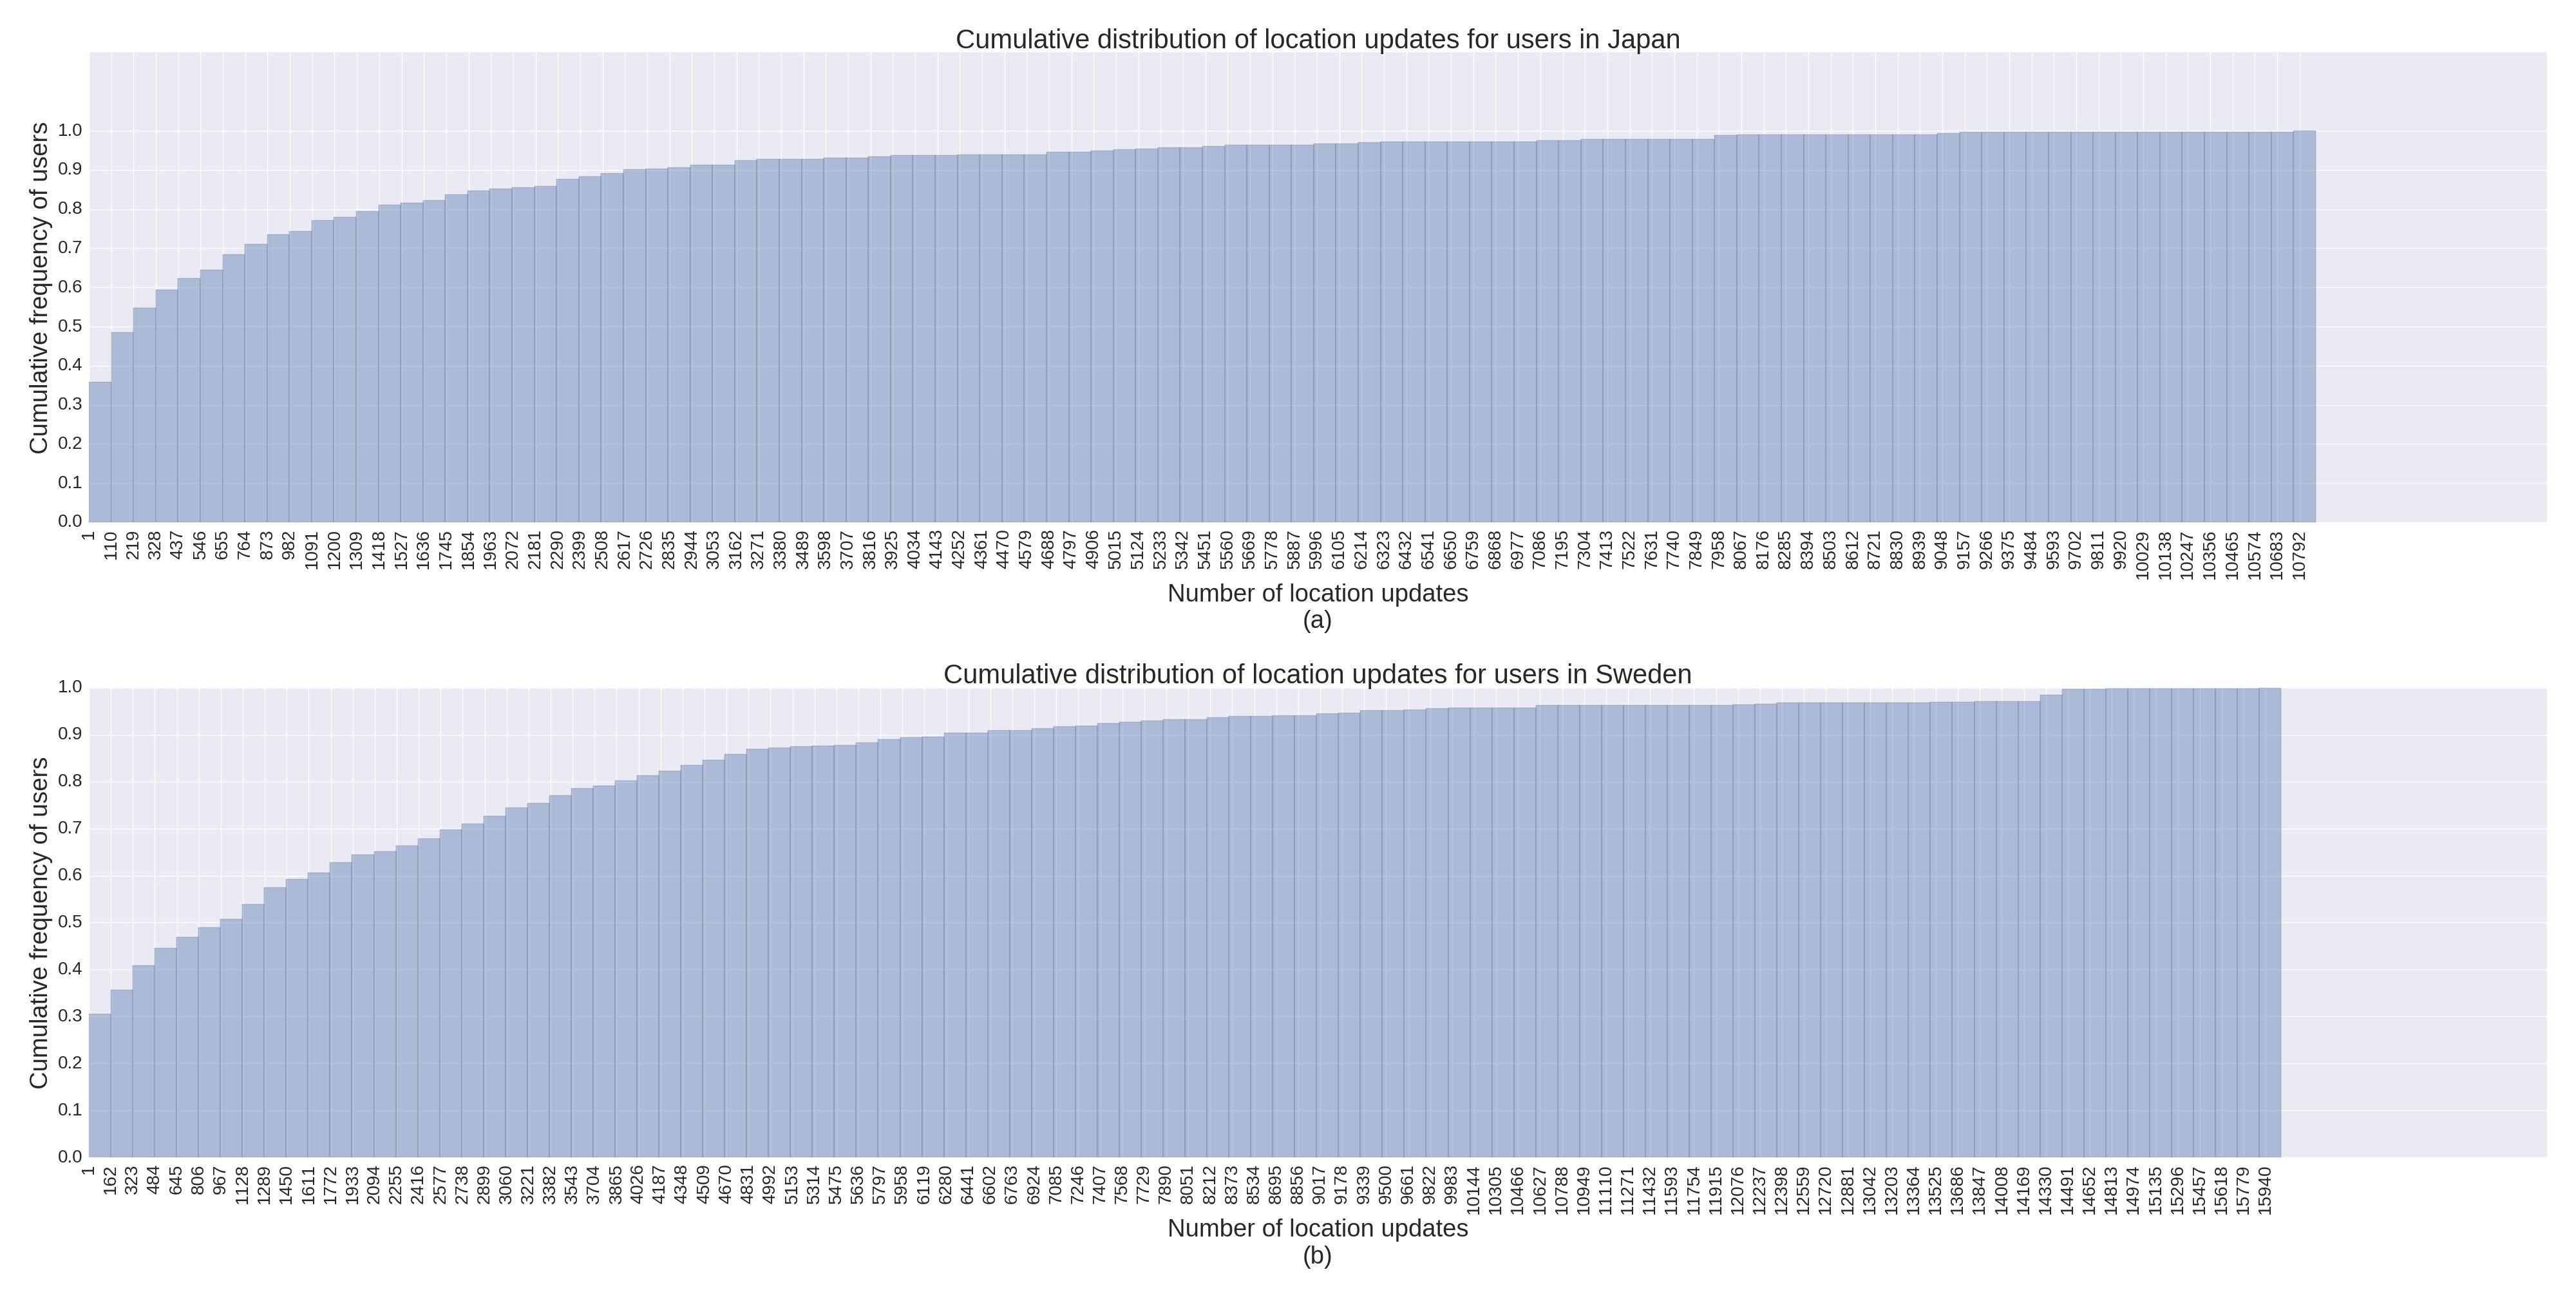
\includegraphics[scale=0.18]{cumulative_dist_loc_updates_swe_jap}
    \caption[Cumulative distribution for location update]{Cumulative distribution for location update. (a) show the cumulative distribution for all users in Japan; (b) show it for Sweden}
    \label{fig:country_cd}
\end{figure}



\begin{figure}[H]
    \centering
    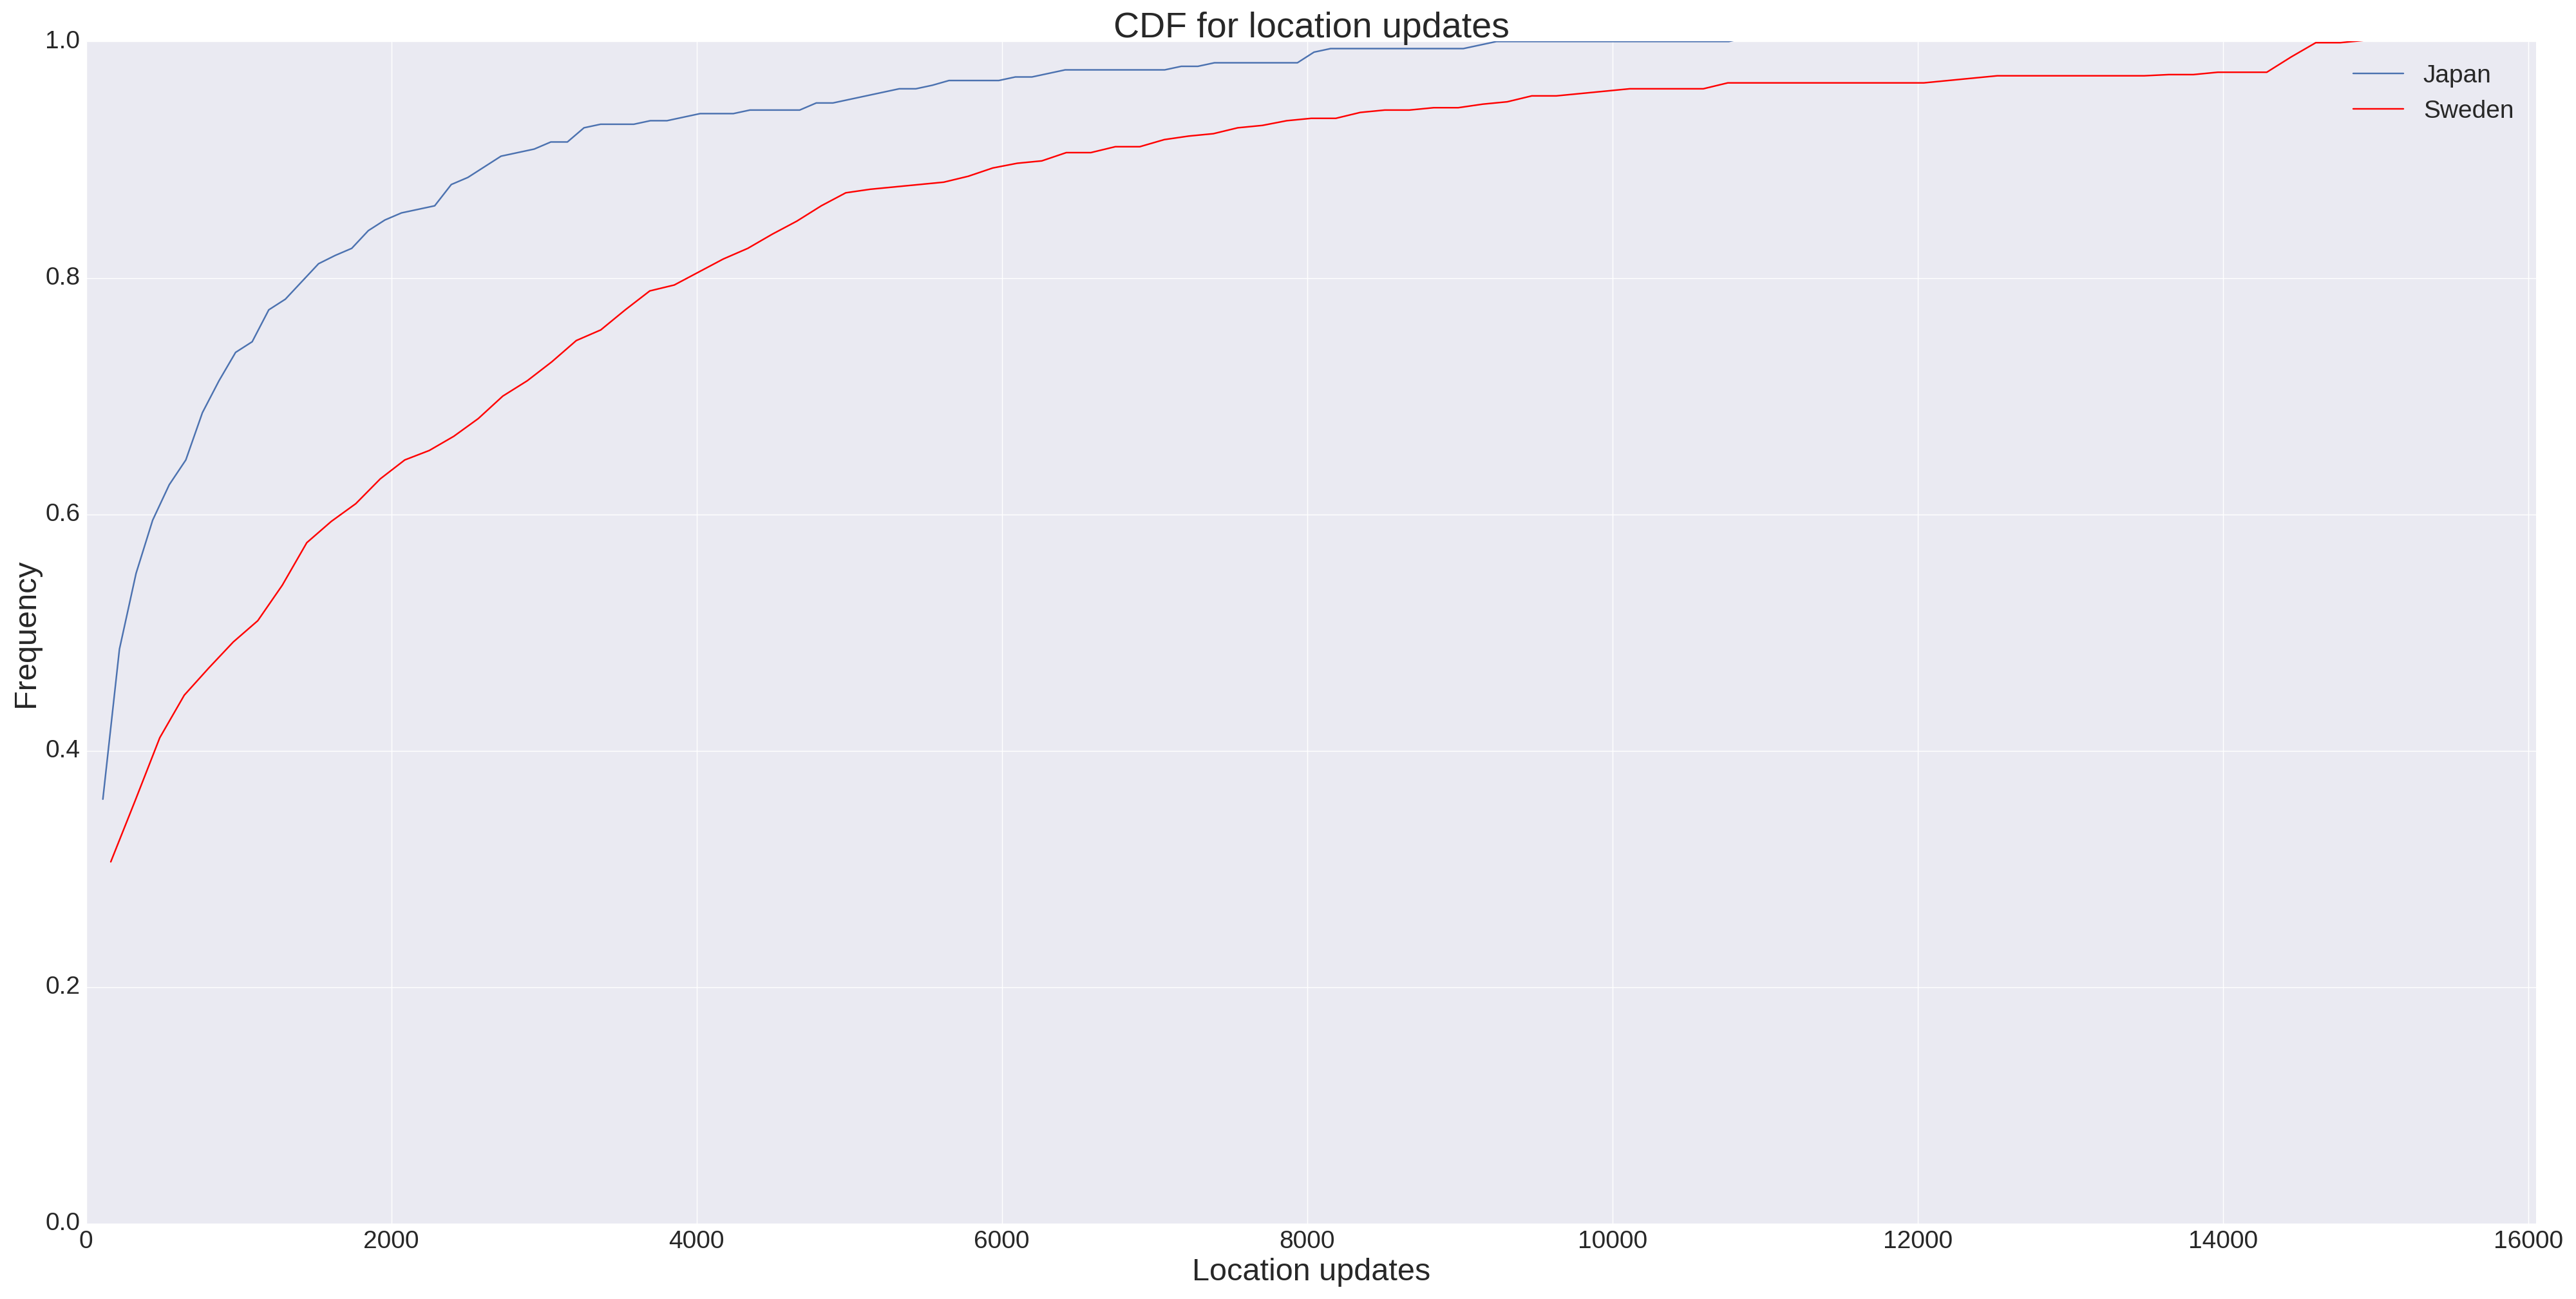
\includegraphics[scale=0.18]{cdf_location_updates_swe_jap}
    \caption{Cumulative Distribution Function (CDF) over location updates for Japan and Sweden}
    \label{fig:country_cdf}
\end{figure}

\begin{table}[htbp]
        \centering
        \small
        \setlength\tabcolsep{2pt}
        \begin{tabular}{|c|c|c|c|c|c|c|c|c|c|c|}
            \hline
                         & Japan      &   Sweden      \\[-3pt]
            \hline
                 Minimum &    0.003       &   0.002          \\
            \hline
                 Q1      &  0.081     &   0.140      \\
            \hline
                 Median  & 0.679     &   1.851      \\
            \hline
                 Mean    &  2.973   &  4.191     \\
            \hline
                 Q3      & 3.330    &   5.855     \\
            \hline
                 Maximum &  32.744 &  28.820     \\
            \hline
                 IQR     &  3.349   &  5.715      \\
            \hline
            
        \end{tabular}
        \caption{Quantiles and mean over location updates for Japan and Sweden per user} %add this between 'caption' and '{...' for new text in listing of tables: [New caption text only for listing of tables]
        \label{tab:stat_loc_updates}
\end{table}


En ting er at kigge på antal lokations opdateringer og se hvordan de er distribueret blandt brugerne i det pågældende land, men det er også interessant at se hvordan opdateringerne er distribueret henover de 3 måneder vi har med at gøre. Er det ligeligt fordelt? Står en enekelt måned for det hele? Er der forskelt på de to lande? Til dette har vi valgt at visualisere dette ved brug af Heatmaps (Figure \ref{fig:heatmap_jap} p.  \pageref{fig:heatmap_jap} and Figure \ref{fig:heatmap_swe} p. \pageref{fig:heatmap_swe}). 
\begin{figure}[H]
    \centering
    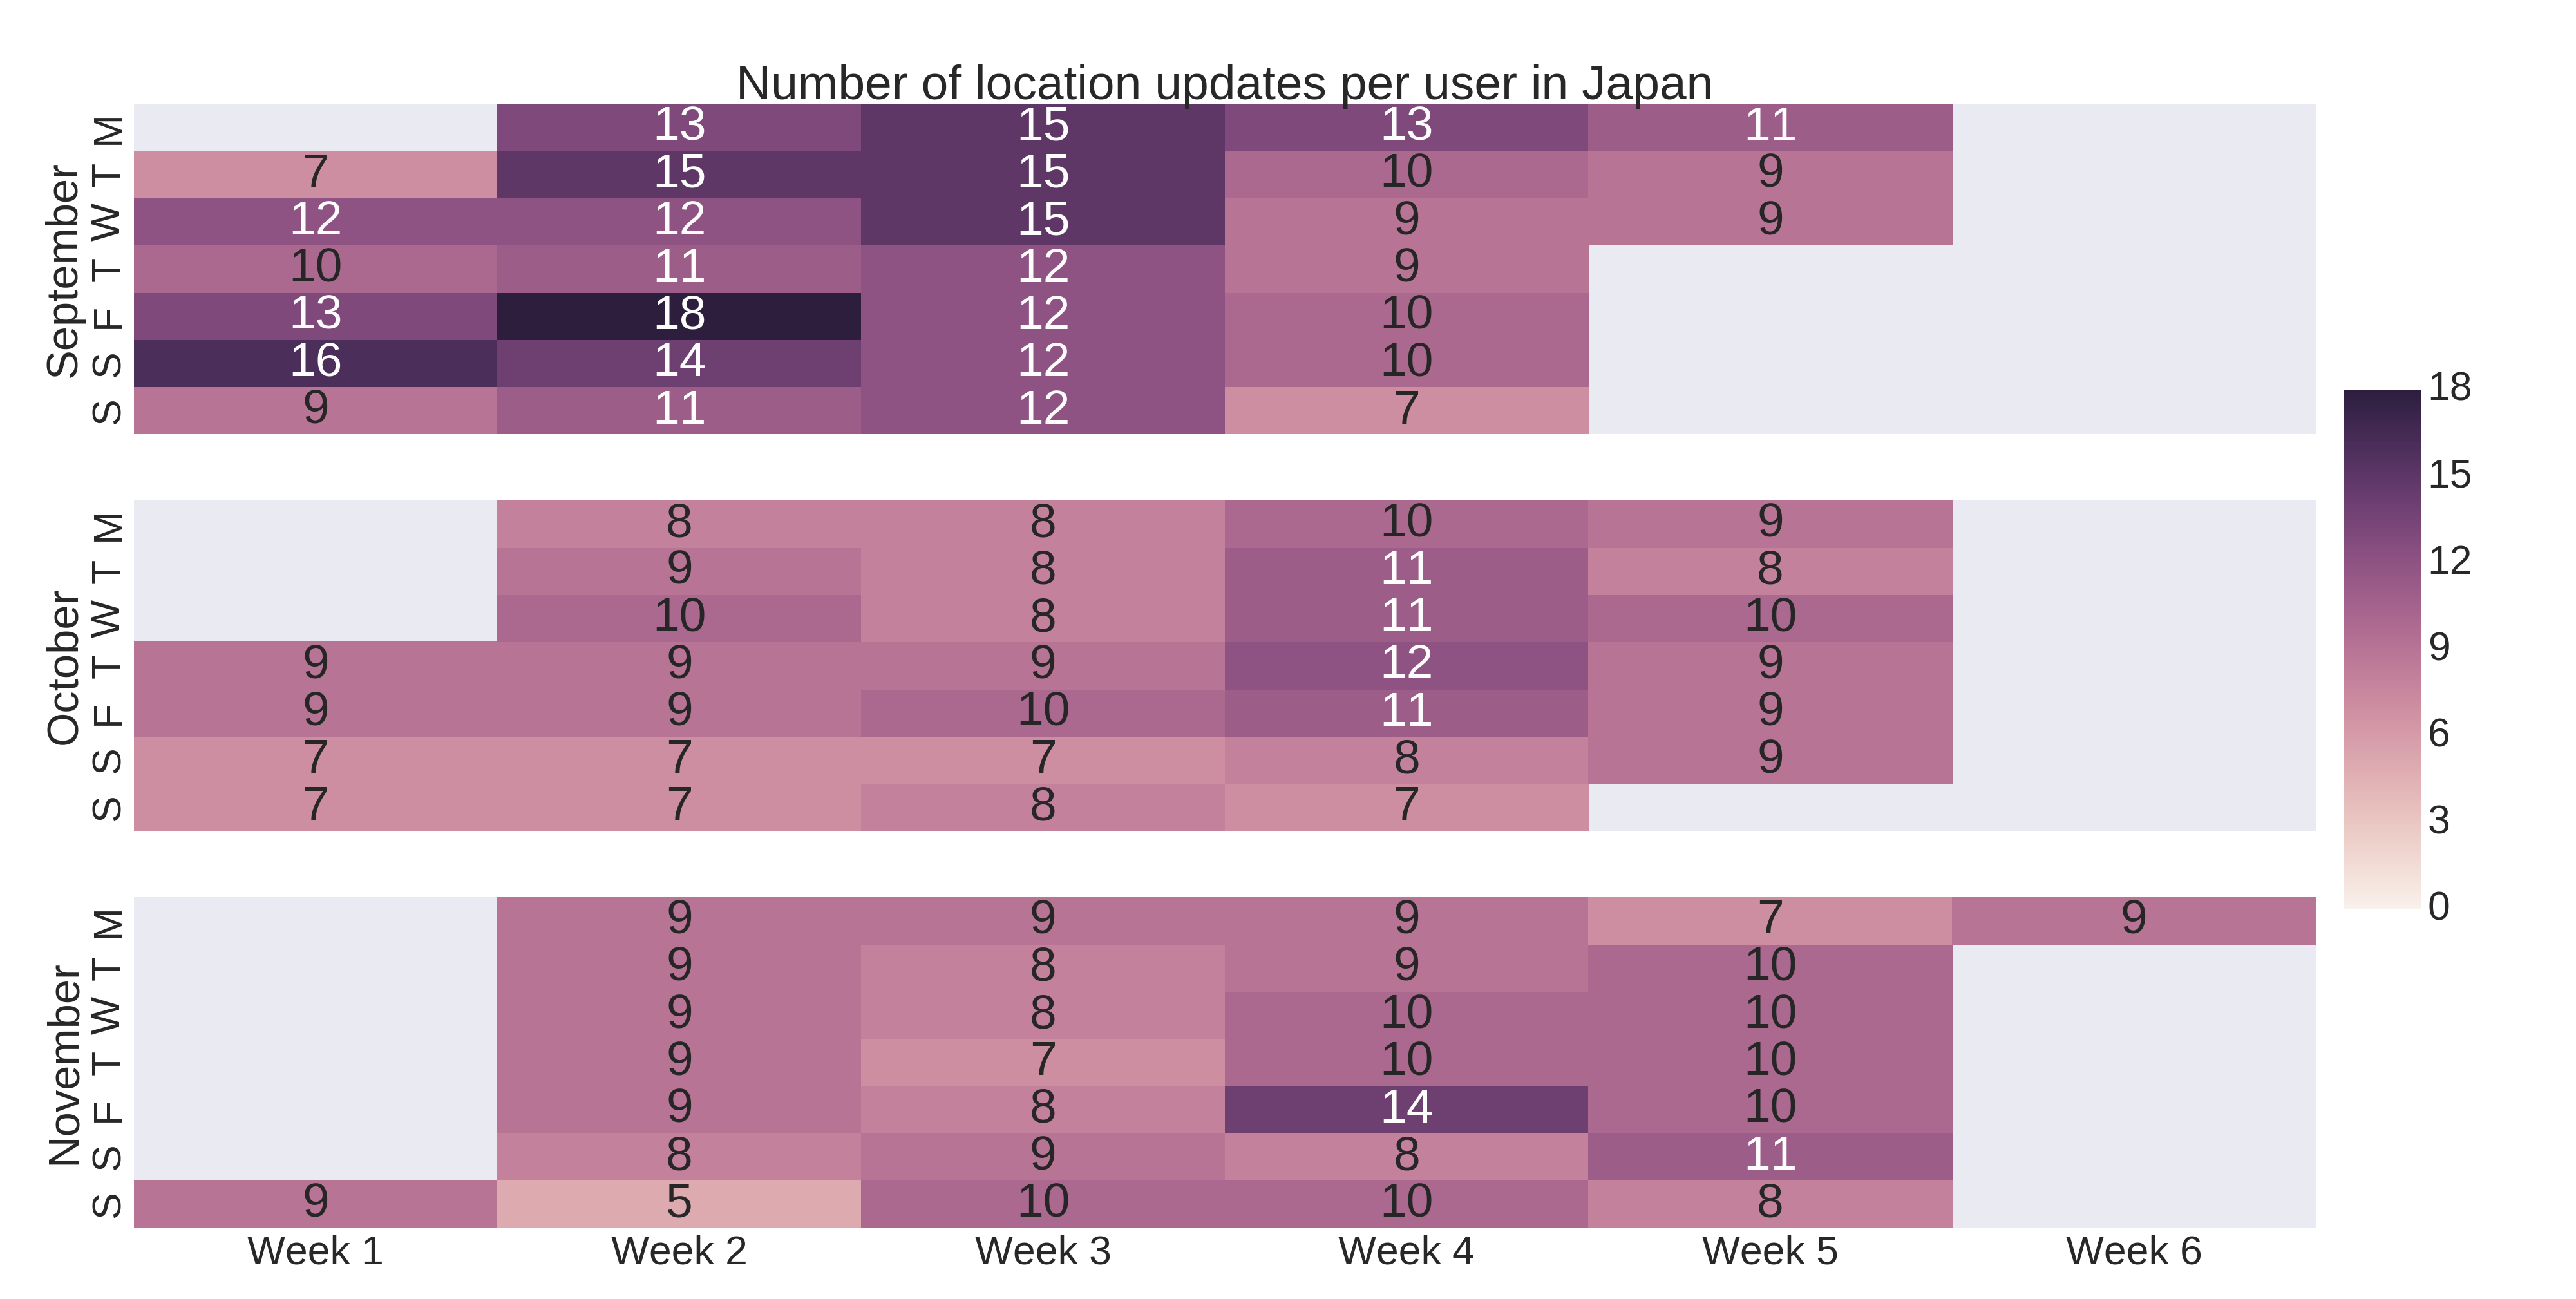
\includegraphics[scale=0.18]{heatmap_location_updates_japan}
    \caption{Heatmap for location updates over the 3 month period in Japan}
    \label{fig:heatmap_jap}
\end{figure}


\begin{figure}[H]
    \centering
    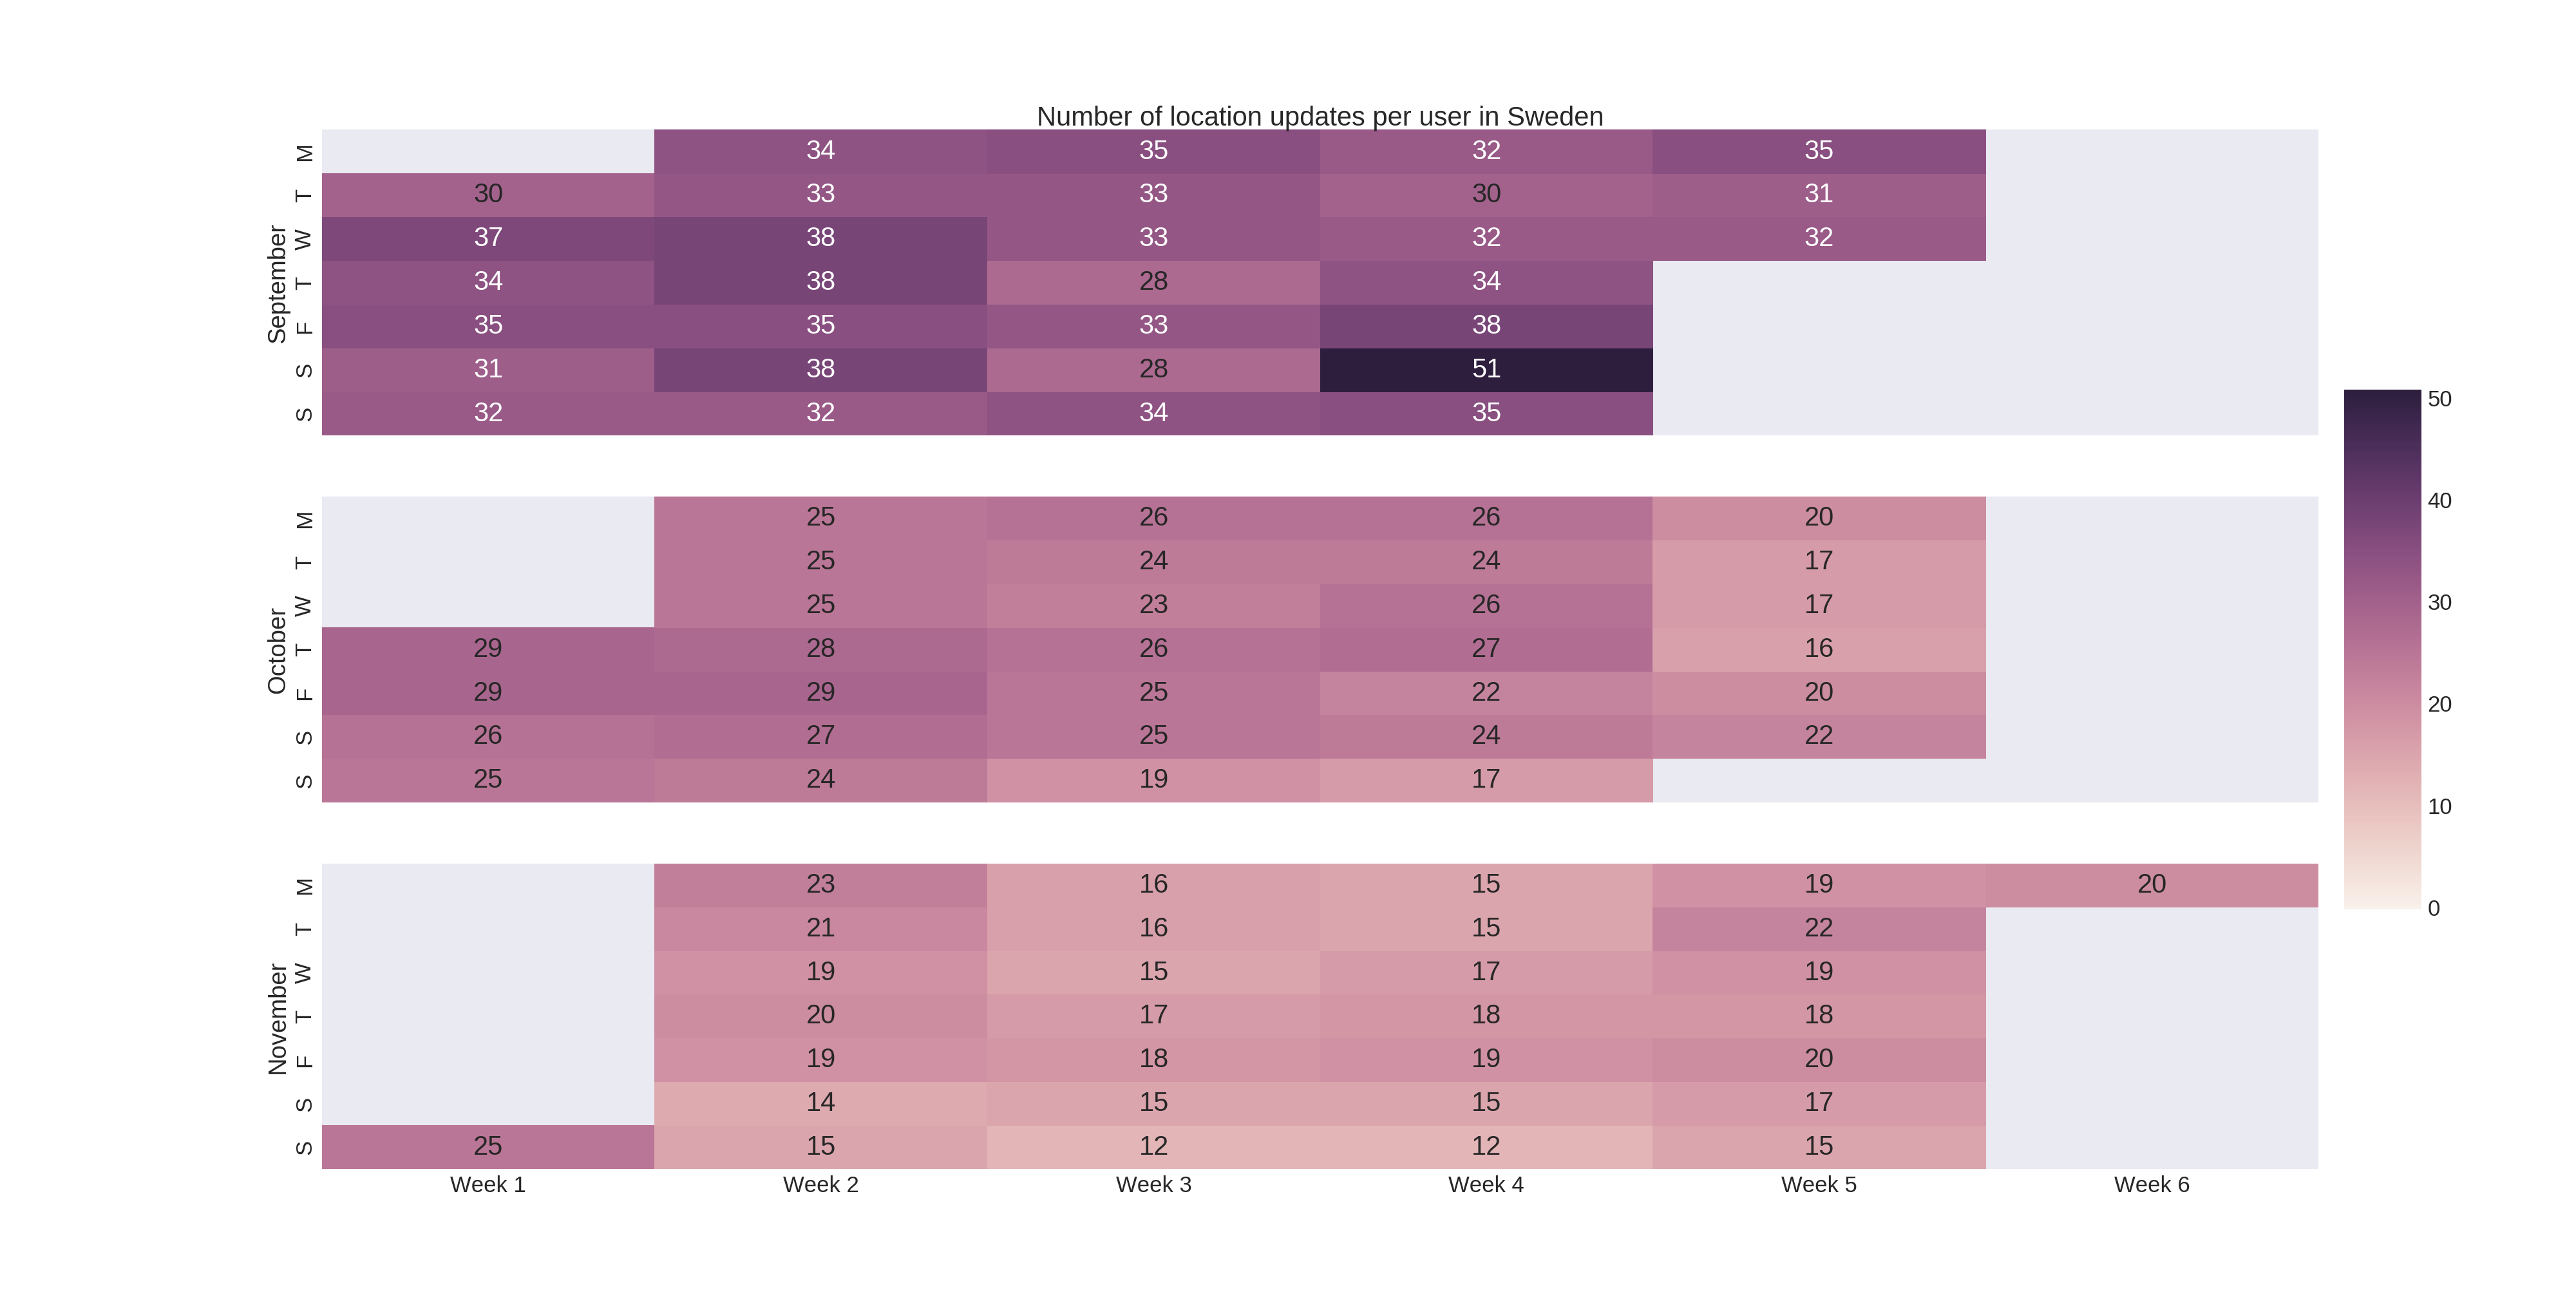
\includegraphics[scale=0.18]{heatmap_location_updates_sweden}
    \caption{Heatmap for location updates over the 3 month period in Sweden}
    \label{fig:heatmap_swe}
\end{figure}



Som man kan er der lidt færrer lande end det vi tidligere skyldtes. Dette 

Our work will focus on the location updates from Japan. There is 332 users in Japan for which we have location updates.
When training our classifier we divided the dataset into three parts where each corresponded to a month.

Japan locations for September: 340198
Japan locations for October: 208242
Japan locations for November: 102442

\textbf{App og homophily del}\\


Over disse 3 måneder blev der indsamlet 2.665.893 geolokation records, som er vores primær data. 
\textcolor{red}{When we got the dataset it was divided into multiple Apache Avro files which is a data serialization framework for Hadoop.\cite{apacheavro}}

